\chapter{Cox Proportional Hazards Model}
\label{cox_proportional_hazards_model}

\section{Introduction}

Many of the clinical and imaging features that were found to be associated with survival in Chapter~\ref{literature_review} were found using the Cox proportional hazards (CPH) model.
CPH is a survival analysis model that is used to investigate the relationship between the time to an event and the factors that may influence it.

As a first step in my investigation into the predictive power of clinical and imaging features in MND, I used a CPH model to investigate the relationship between the time to death and the clinical and neuroimaging features that were extracted from the ALS Biomarkers Study and Ospedale San Raffaele MND cohorts.

Previously, Querin and colleagues used a multivariable CPH to compare the predictive power of clinical and spinal cord imaging features in ALS in a cohort of 49 ALS patients, and concluded that spinal MRI measures were more predictive than clinical measures~\cite{querinSpinalCordMultiparametric2017}.
In this chapter, univariable, unimodal multivariable, and multimodal multivariable CPH models were used to investigate the relationship between the time to death and the clinical and imaging features in a larger cohort of 125 MND patients.

%\begin{itemize}
%    \item Cox proportional hazards model - what is it?
%    \item What is my hypothesis: using clinical and imaging features together in a simple cox regression will need to hugher concordance than imaging and clinical data alone
%    \item What is concordance? How is it calculated?
%    \item Examples of cox models in ALS before:
%\end{itemize}

\section{Data}

Data from two studies was used for this survival analysis: ALS Biomarkers Study and Opsedale San Raffaele.
Both of these datasets contain clinical information on MND patients and structural imaging conducted during their disease course.

The outcome of interest in this analysis is time to death, censored by date of censorship if recorded in the dataset or date of last data update if not.
The Ospedale San Raffaele cohort defines their endpoint as death or tracheostomy, but the ALS Biomarkers Study only defines their endpoint as death.

The clinical features in this study are the patient's sex, baseline ALSFRS-R, diagnostic delay, age at diagnosis, site of onset (categorised as bulbar and non-bulbar), signs of FTD, and their MND subtype (categorised as ALS and non-ALS).
These features were chosen for their clinical relevance to survival in MND and their availability in both datasets.

Patients were excluded if they did not have a T1- or T2-weighted MRI within 12 months before or after an MND diagnosis.
Regional brain volumes were extracted from the MRI using SynthSeg~\cite{billotSynthSegDomainRandomisation2021}, a modality-agnostic deep-learning segmentation tool.
A modality agnostic tool was chosen to overcome the inconsistency in MRI protocols within the ALS Biomarkers Study and between the ALS Biomarkers Study and Ospedale San Raffaele's MND cohort.
The dimensionality of the 33 regions was reduced to 12 by summing right and left regions and choosing regions relevant to MND pathology.
The remaining regions were z-score normalised.

\begin{table}
\centering
\caption{Demographics and clinical characteristics of the patients included in the analysis. ALSFRSr: ALS Functional Rating Scale-Revised.}
\label{tab:coxdemographics}
\begin{tabular}{|ll|}
\hline
              \textbf{Variable}                          &      \\
\hline
 n                               & 125         \\\hline
 Sex, n (\%)          & \\
 \hspace{5mm}Female & 55 (44.0)   \\
\hspace{5mm}Male & 70 (56.0)   \\\hline
 ALSFRSr, mean (SD)                 & 38.9 (6.4)  \\\hline
 Survival (months), mean (SD)         & 34.3 (27.3) \\\hline
 Diagnostic Delay (months), mean (SD)  & 13.6 (13.2) \\\hline
 Age at Diagnosis (years), mean (SD)  & 62.6 (11.4) \\\hline
 Site of Onset, n (\%)        &  \\
 \hspace{5mm}Non-bulbar   & 91 (72.8)   \\
 \hspace{5mm}Bulbar  & 34 (27.2)   \\\hline
 Frontotemporal Dementia, n (\%)       & \\
 \hspace{5mm}Not present & 87 (69.6)   \\
\hspace{5mm}Present & 38 (30.4)   \\\hline
 MND Type, n (\%)                & \\
 \hspace{5mm}Not ALS   & 21 (16.8)   \\
 \hspace{5mm}ALS   & 104 (83.2)  \\\hline
 Outcome, n (\%)                          & \\
 \hspace{5mm}Censored   & 21 (16.8)   \\
\hspace{5mm}Died   & 104 (83.2)  \\\hline

\end{tabular}
\end{table}

The demographics and clinical characteristics of the patients who were included in the analysis are shown in Table~\ref{tab:coxdemographics}.
Out of the 125 patients, 21 were censored and 104 died during the study period.
Censored patients were those who were still alive at the end of the study period (or at the time of data download: 5th March 2024) or who were lost to follow-up before the end of the study period.

\section{Methods}

A CPH model is expressed as
\begin{equation}\label{eq:coxhazard}
    h(t) = h_0(t) \exp{(\beta_1 X_1 + \beta_2 X_2 + ... + \beta_n X_n)},
\end{equation}
where $t$ is the survival time, $h(t)$ is the hazard function, $\bold{X}$ are the variables investigated, $h_0(t)$ is the baseline hazard if all the variables were 0.
The hazard ratios (HRs) are represented as $\beta$, with $\beta_1$ being the hazard ratio for the variable $X_1$.
A HR larger than 1 indicates the variable is associated with a poorer prognosis, or increased risk of the event, which is death in this CPH application.
The assumption of proportional hazards is that each individual in the analysis has the same hazard function, but the hazard functions are scaled by a constant factor, which is not dependent on time.
The Python package, lifelines, was used to implement the CPH models and to test the proportional hazards assumption (citation here).
Since the aim of this analysis was to see how multimodal data affects survival analysis of MND, four models were run:
\begin{enumerate}
\setlength\itemsep{-0.5em}
    \item Univariable model: each feature was tested individually to see if it was associated with survival without adjusting for other features.
    \item Clinical-only model: multivariable model with only clinical features.
    \item Imaging-only model: multivariable model with only imaging features.
    \item Clinical and imaging model: multivariable model with both clinical and imaging features.
\end{enumerate}

%The models we used were not stratified by any variables, as the sample size was relatively small and stratifying the model may lead to less informative results than just including the features and acknowledging the violation of the proportional hazards assumption.

The CPH models estimated the hazard ratios and their 95\% confidence intervals for each variable, with significance level set at $p<0.05$.

The quality of models fit to the data was assessed using the concordance index, which is a measure of how well the model predicts the order of the survival times, and the Akaike Information Criterion (AIC), which is a measure of the model's goodness of fit balanced with its complexity.

\section{Results}

\subsection{Univariable}

% \begin{table}
% \centering
% % \resizebox{1.2\linewidth}{!}{%
% \begin{sidewaystable}
% \begin{tabular}{|l|ll|ll|ll|ll|} 
% \cline{2-9}
% \multicolumn{1}{l|}{} & \multicolumn{2}{l|}{\multirow{2}{*}{Univariable}} & \multicolumn{6}{l|}{Multivariable} \\ 
% \cline{4-9}
% \multicolumn{1}{l|}{} & \multicolumn{2}{l|}{} & \multicolumn{2}{l|}{Clinical} & \multicolumn{2}{l|}{Imaging} & \multicolumn{2}{l|}{Multimodal} \\ 
% \hline
% Variable & HR (95\% CI) & $p$ & HR (95\% CI) & $p$ & HR (95\% CI) & $p$ & HR (95\% CI) & $p$ \\ 
% \hline
% Sex &  &  &  &  & {\cellcolor[rgb]{0.753,0.753,0.753}} & {\cellcolor[rgb]{0.753,0.753,0.753}} &  &  \\
% Female & 1.00, Ref & - & 1.00, Ref & - & {\cellcolor[rgb]{0.753,0.753,0.753}} & {\cellcolor[rgb]{0.753,0.753,0.753}} & 1.00, Ref & - \\
% Male & 0.91 (0.62--1.34) & 0.6417 & \textcolor[rgb]{0.2,0.2,0.2}{1.13 (0.72 -- 1.77)} & \textcolor[rgb]{0.2,0.2,0.2}{0.5995} & {\cellcolor[rgb]{0.753,0.753,0.753}} & {\cellcolor[rgb]{0.753,0.753,0.753}} & \textcolor[rgb]{0.2,0.2,0.2}{1.11 (0.62 -- 1.99)} & \textcolor[rgb]{0.2,0.2,0.2}{0.7315} \\ 
% \hline
% ALSFRS-R & 0.70 (0.60--0.82) & \begin{tabular}[c]{@{}l@{}}$<$\textbf{\textbf{0.0001}}\\\end{tabular} & \textcolor[rgb]{0.2,0.2,0.2}{0.62 (0.51 -- 0.76)} & $<$\textbf{0.0001} & {\cellcolor[rgb]{0.753,0.753,0.753}} & {\cellcolor[rgb]{0.753,0.753,0.753}} & \textcolor[rgb]{0.2,0.2,0.2}{0.68 (0.53 -- 0.88)} & \textcolor[rgb]{0.2,0.2,0.2}{\textbf{0.0034}} \\ 
% \hline
% Diagnostic delay, mo & 0.77 (0.60--0.99) & \textbf{0.0409} & \textcolor[rgb]{0.2,0.2,0.2}{0.79 (0.59 -- 1.06)} & \textcolor[rgb]{0.2,0.2,0.2}{0.1165} & {\cellcolor[rgb]{0.753,0.753,0.753}} & {\cellcolor[rgb]{0.753,0.753,0.753}} & \textcolor[rgb]{0.2,0.2,0.2}{0.86 (0.63 -- 1.18)} & \textcolor[rgb]{0.2,0.2,0.2}{0.3500} \\ 
% \hline
% Age at diagnosis, yr & 1.48 (1.29--1.84) & \textbf{0.0005} & \textcolor[rgb]{0.2,0.2,0.2}{1.53 (1.23 -- 1.92)} & \textcolor[rgb]{0.2,0.2,0.2}{\textbf{0.0002}} & {\cellcolor[rgb]{0.753,0.753,0.753}} & {\cellcolor[rgb]{0.753,0.753,0.753}} & \textcolor[rgb]{0.2,0.2,0.2}{1.19 (0.84 -- 1.67)} & \textcolor[rgb]{0.2,0.2,0.2}{0.3265} \\ 
% \hline
% Site of onset &  &  &  &  & {\cellcolor[rgb]{0.753,0.753,0.753}} & {\cellcolor[rgb]{0.753,0.753,0.753}} &  &  \\
% Non-bulbar & 1.00, Ref & - & 1.00, Ref & - & {\cellcolor[rgb]{0.753,0.753,0.753}} & {\cellcolor[rgb]{0.753,0.753,0.753}} & 1.00, Ref & - \\
% Bulbar & 1.36 (0.88--2.10) & 0.1605 & \textcolor[rgb]{0.2,0.2,0.2}{0.90 (0.55 -- 1.47)} & \textcolor[rgb]{0.2,0.2,0.2}{0.6695} & {\cellcolor[rgb]{0.753,0.753,0.753}} & {\cellcolor[rgb]{0.753,0.753,0.753}} & \textcolor[rgb]{0.2,0.2,0.2}{0.94 (0.54 -- 1.64)} & \textcolor[rgb]{0.2,0.2,0.2}{0.8280} \\ 
% \hline
% FTD &  &  &  &  & {\cellcolor[rgb]{0.753,0.753,0.753}} & {\cellcolor[rgb]{0.753,0.753,0.753}} &  &  \\
% No & 1.00, Ref & - & 1.00, Ref & - & {\cellcolor[rgb]{0.753,0.753,0.753}} & {\cellcolor[rgb]{0.753,0.753,0.753}} & 1.00, Ref & - \\
% Yes & 1.58 (1.04--2.41) & \textbf{0.0337} & \textcolor[rgb]{0.2,0.2,0.2}{1.46 (0.91 -- 2.35)} & \textcolor[rgb]{0.2,0.2,0.2}{0.1152} & {\cellcolor[rgb]{0.753,0.753,0.753}} & {\cellcolor[rgb]{0.753,0.753,0.753}} & \textcolor[rgb]{0.2,0.2,0.2}{1.20 (0.69 -- 2.08)} & \textcolor[rgb]{0.2,0.2,0.2}{0.5177} \\ 
% \hline
% MND Subtype &  &  &  &  & {\cellcolor[rgb]{0.753,0.753,0.753}} & {\cellcolor[rgb]{0.753,0.753,0.753}} &  &  \\
% Non-ALS & 1.00, Ref & - & 1.00, Ref & - & {\cellcolor[rgb]{0.753,0.753,0.753}} & {\cellcolor[rgb]{0.753,0.753,0.753}} & 1.00, Ref & - \\
% ALS & 2.40 (1.36--4.23) & \textbf{0.0026} & \textcolor[rgb]{0.2,0.2,0.2}{1.96 (1.04 -- 3.71)} & \textcolor[rgb]{0.2,0.2,0.2}{\textbf{0.0384}} & {\cellcolor[rgb]{0.753,0.753,0.753}} & {\cellcolor[rgb]{0.753,0.753,0.753}} & \textcolor[rgb]{0.2,0.2,0.2}{2.32 (1.10 -- 4.88)} & \textcolor[rgb]{0.2,0.2,0.2}{\textbf{0.0264}} \\ 
% \hline
% Brain stem & \textcolor[rgb]{0.2,0.2,0.2}{0.66 (0.53 -- 0.83)} & \textcolor[rgb]{0.2,0.2,0.2}{\textbf{0.0003}} & {\cellcolor[rgb]{0.753,0.753,0.753}} & {\cellcolor[rgb]{0.753,0.753,0.753}} & \textcolor[rgb]{0.2,0.2,0.2}{0.64 (0.41 -- 1.01)} & \textcolor[rgb]{0.2,0.2,0.2}{0.0557} & \textcolor[rgb]{0.2,0.2,0.2}{0.64 (0.38 -- 1.08)} & \textcolor[rgb]{0.2,0.2,0.2}{0.0958} \\ 
% \hline
% CSF & \textcolor[rgb]{0.2,0.2,0.2}{1.40 (1.16 -- 1.70)} & \textcolor[rgb]{0.2,0.2,0.2}{\textbf{0.0005}} & {\cellcolor[rgb]{0.753,0.753,0.753}} & {\cellcolor[rgb]{0.753,0.753,0.753}} & \textcolor[rgb]{0.2,0.2,0.2}{1.10 (0.79 -- 1.54)} & \textcolor[rgb]{0.2,0.2,0.2}{0.5794} & \textcolor[rgb]{0.2,0.2,0.2}{0.93 (0.61 -- 1.43)} & \textcolor[rgb]{0.2,0.2,0.2}{0.7370} \\ 
% \hline
% Lateral ventricles & \textcolor[rgb]{0.2,0.2,0.2}{1.58 (1.32 -- 1.89)} & \textbf{$<$0.0001} & {\cellcolor[rgb]{0.753,0.753,0.753}} & {\cellcolor[rgb]{0.753,0.753,0.753}} & \textcolor[rgb]{0.2,0.2,0.2}{1.52 (1.06 -- 2.17)} & \textcolor[rgb]{0.2,0.2,0.2}{\textbf{0.0214}} & \textcolor[rgb]{0.2,0.2,0.2}{1.47 (0.96 -- 2.24)} & \textcolor[rgb]{0.2,0.2,0.2}{0.0731} \\ 
% \hline
% Hippocampus & \textcolor[rgb]{0.2,0.2,0.2}{0.59 (0.47 -- 0.73)} & \textbf{$<$0.0001} & {\cellcolor[rgb]{0.753,0.753,0.753}} & {\cellcolor[rgb]{0.753,0.753,0.753}} & \textcolor[rgb]{0.2,0.2,0.2}{0.96 (0.58 -- 1.61)} & \textcolor[rgb]{0.2,0.2,0.2}{0.8811} & \textcolor[rgb]{0.2,0.2,0.2}{1.18 (0.67 -- 2.08)} & \textcolor[rgb]{0.2,0.2,0.2}{0.5663} \\ 
% \hline
% Amygdala & \textcolor[rgb]{0.2,0.2,0.2}{0.59 (0.47 -- 0.73)} & \textbf{$<$0.0001} & {\cellcolor[rgb]{0.753,0.753,0.753}} & {\cellcolor[rgb]{0.753,0.753,0.753}} & \textcolor[rgb]{0.2,0.2,0.2}{0.65 (0.42 -- 1.00)} & \textcolor[rgb]{0.2,0.2,0.2}{0.0502} & \textcolor[rgb]{0.2,0.2,0.2}{0.68 (0.43 -- 1.07)} & \textcolor[rgb]{0.2,0.2,0.2}{0.0927} \\ 
% \hline
% Thalamus & \textcolor[rgb]{0.2,0.2,0.2}{0.78 (0.64 -- 0.96)} & \textcolor[rgb]{0.2,0.2,0.2}{\textbf{0.0173}} & {\cellcolor[rgb]{0.753,0.753,0.753}} & {\cellcolor[rgb]{0.753,0.753,0.753}} & \textcolor[rgb]{0.2,0.2,0.2}{1.30 (0.79 -- 2.14)} & \textcolor[rgb]{0.2,0.2,0.2}{0.2931} & \textcolor[rgb]{0.2,0.2,0.2}{1.14 (0.67 -- 1.93)} & \textcolor[rgb]{0.2,0.2,0.2}{0.6229} \\ 
% \hline
% Caudate & \textcolor[rgb]{0.2,0.2,0.2}{0.77 (0.64 -- 0.93)} & \textcolor[rgb]{0.2,0.2,0.2}{\textbf{0.0052}} & {\cellcolor[rgb]{0.753,0.753,0.753}} & {\cellcolor[rgb]{0.753,0.753,0.753}} & \textcolor[rgb]{0.2,0.2,0.2}{0.62 (0.41 -- 0.94)} & \textcolor[rgb]{0.2,0.2,0.2}{\textbf{0.0245}} & \textcolor[rgb]{0.2,0.2,0.2}{0.69 (0.43 -- 1.11)} & \textcolor[rgb]{0.2,0.2,0.2}{0.1253} \\ 
% \hline
% Putamen & \textcolor[rgb]{0.2,0.2,0.2}{0.72 (0.60 -- 0.87)} & \textcolor[rgb]{0.2,0.2,0.2}{\textbf{0.0007}} & {\cellcolor[rgb]{0.753,0.753,0.753}} & {\cellcolor[rgb]{0.753,0.753,0.753}} & \textcolor[rgb]{0.2,0.2,0.2}{1.30 (0.71 -- 2.37)} & \textcolor[rgb]{0.2,0.2,0.2}{0.3884} & \textcolor[rgb]{0.2,0.2,0.2}{0.88 (0.47 -- 1.66)} & \textcolor[rgb]{0.2,0.2,0.2}{0.6932} \\ 
% \hline
% Pallidum & \textcolor[rgb]{0.2,0.2,0.2}{0.75 (0.61 -- 0.91)} & \textcolor[rgb]{0.2,0.2,0.2}{\textbf{0.0041}} & {\cellcolor[rgb]{0.753,0.753,0.753}} & {\cellcolor[rgb]{0.753,0.753,0.753}} & \textcolor[rgb]{0.2,0.2,0.2}{0.75 (0.50 -- 1.14)} & \textcolor[rgb]{0.2,0.2,0.2}{0.1819} & \textcolor[rgb]{0.2,0.2,0.2}{0.87 (0.57 -- 1.32)} & \textcolor[rgb]{0.2,0.2,0.2}{0.5007} \\ 
% \hline
% Cerebral white matter & \textcolor[rgb]{0.2,0.2,0.2}{0.99 (0.82 -- 1.20)} & \textcolor[rgb]{0.2,0.2,0.2}{0.9339} & {\cellcolor[rgb]{0.753,0.753,0.753}} & {\cellcolor[rgb]{0.753,0.753,0.753}} & \textcolor[rgb]{0.2,0.2,0.2}{2.35 (1.16 -- 4.77)} & \textcolor[rgb]{0.2,0.2,0.2}{\textbf{0.0181}} & \textcolor[rgb]{0.2,0.2,0.2}{2.43 (1.16 -- 5.10)} & \textcolor[rgb]{0.2,0.2,0.2}{\textbf{0.0185}} \\ 
% \hline
% Cerebellum white matter & \textcolor[rgb]{0.2,0.2,0.2}{0.83 (0.67 -- 1.02)} & \textcolor[rgb]{0.2,0.2,0.2}{0.0775} & {\cellcolor[rgb]{0.753,0.753,0.753}} & {\cellcolor[rgb]{0.753,0.753,0.753}} & \textcolor[rgb]{0.2,0.2,0.2}{0.97 (0.56 -- 1.66)} & \textcolor[rgb]{0.2,0.2,0.2}{0.9054} & \textcolor[rgb]{0.2,0.2,0.2}{1.14 (0.63 -- 2.05)} & \textcolor[rgb]{0.2,0.2,0.2}{0.6714} \\ 
% \hline
% Cerebellum cortex & \textcolor[rgb]{0.2,0.2,0.2}{0.71 (0.57 -- 0.88)} & \textcolor[rgb]{0.2,0.2,0.2}{\textbf{0.0016}} & {\cellcolor[rgb]{0.753,0.753,0.753}} & {\cellcolor[rgb]{0.753,0.753,0.753}} & \textcolor[rgb]{0.2,0.2,0.2}{0.79 (0.52 -- 1.21)} & \textcolor[rgb]{0.2,0.2,0.2}{0.2888} & \textcolor[rgb]{0.2,0.2,0.2}{0.82 (0.51 -- 1.32)} & \textcolor[rgb]{0.2,0.2,0.2}{0.4135} \\ 
% \hline
% Cerebral cortex & \textcolor[rgb]{0.2,0.2,0.2}{0.99 (0.82 -- 1.21)} & \textcolor[rgb]{0.2,0.2,0.2}{0.9462} & {\cellcolor[rgb]{0.753,0.753,0.753}} & {\cellcolor[rgb]{0.753,0.753,0.753}} & \textcolor[rgb]{0.2,0.2,0.2}{0.90 (0.45 -- 1.83)} & \textcolor[rgb]{0.2,0.2,0.2}{0.7769} & \textcolor[rgb]{0.2,0.2,0.2}{0.87 (0.41 -- 1.84)} & \textcolor[rgb]{0.2,0.2,0.2}{0.7118} \\
% \hline
% \end{tabular}
% \end{sidewaystable}

% \end{table}

% Please add the following required packages to your document preamble:
% \usepackage{multirow}
% \usepackage{graphicx}
% \usepackage[table,xcdraw]{xcolor}
% Beamer presentation requires \usepackage{colortbl} instead of \usepackage[table,xcdraw]{xcolor}
% \usepackage{multirow}
% \usepackage{colortbl}
% \usepackage{rotating}

\begin{sidewaystable}
{\small\setlength{\tabcolsep}{4pt}
\centering
\caption{Hazard ratios of survival risk in patients with motor neuron disease for univariable and three multivariable Cox proportional hazards regressions: clinical only, imaging-features only, and clinical and imaging features together (multimodal). Acronyms: FTD - frontotemporal dementia, ALSFRS-R - revised amytrophic lateral sclerosis functional rating scale, CSF - cerebrospinal fluid.}
\label{tab:allfeatures_cox}
\begin{tabular}{|l|lr|lr|lr|lr|} 
\cline{2-9}
\multicolumn{1}{l|}{} & \multicolumn{2}{l|}{\multirow{2}{*}{Univariable}} & \multicolumn{6}{c|}{Multivariable} \\ 
\cline{4-9}
\multicolumn{1}{l|}{} & \multicolumn{2}{l|}{} & \multicolumn{2}{l|}{Clinical} & \multicolumn{2}{l|}{Imaging} & \multicolumn{2}{l|}{Multimodal} \\ 
\hline
Variable & HR (95\% CI) & $p$ & HR (95\% CI) & $p$ & HR (95\% CI) & $p$ & HR (95\% CI) & $p$ \\ \hline
\multicolumn{1}{|l}{\textbf{Clinical}} &  & \multicolumn{1}{l}{} &  & \multicolumn{1}{l}{} &  & \multicolumn{1}{l}{} &  &  \\ 
\hline
Sex &  &  &  &  & {\cellcolor[rgb]{0.753,0.753,0.753}} & {\cellcolor[rgb]{0.753,0.753,0.753}} &  &  \\
\hspace{5mm}Female & 1.00, Ref & - & 1.00, Ref & - & {\cellcolor[rgb]{0.753,0.753,0.753}} & {\cellcolor[rgb]{0.753,0.753,0.753}} & 1.00, Ref & - \\
\hspace{5mm}Male & 0.91 (0.62--1.34) & 0.6417 & \textcolor[rgb]{0.2,0.2,0.2}{1.13 (0.72 -- 1.77)} & \textcolor[rgb]{0.2,0.2,0.2}{0.5995} & {\cellcolor[rgb]{0.753,0.753,0.753}} & {\cellcolor[rgb]{0.753,0.753,0.753}} & \textcolor[rgb]{0.2,0.2,0.2}{1.11 (0.62 -- 1.99)} & \textcolor[rgb]{0.2,0.2,0.2}{0.7315} \\ 
\hline
ALSFRS-R & 0.70 (0.60--0.82) & \begin{tabular}[c]{@{}l@{}}$<$\textbf{\textbf{0.0001}}\\\end{tabular} & \textcolor[rgb]{0.2,0.2,0.2}{0.62 (0.51 -- 0.76)} & $<$\textbf{0.0001} & {\cellcolor[rgb]{0.753,0.753,0.753}} & {\cellcolor[rgb]{0.753,0.753,0.753}} & \textcolor[rgb]{0.2,0.2,0.2}{0.68 (0.53 -- 0.88)} & \textcolor[rgb]{0.2,0.2,0.2}{\textbf{0.0034}} \\ 
\hline
Diagnostic delay, mo & 0.77 (0.60--0.99) & \textbf{0.0409} & \textcolor[rgb]{0.2,0.2,0.2}{0.79 (0.59 -- 1.06)} & \textcolor[rgb]{0.2,0.2,0.2}{0.1165} & {\cellcolor[rgb]{0.753,0.753,0.753}} & {\cellcolor[rgb]{0.753,0.753,0.753}} & \textcolor[rgb]{0.2,0.2,0.2}{0.86 (0.63 -- 1.18)} & \textcolor[rgb]{0.2,0.2,0.2}{0.3500} \\ 
\hline
Age at diagnosis, yr & 1.48 (1.29--1.84) & \textbf{0.0005} & \textcolor[rgb]{0.2,0.2,0.2}{1.53 (1.23 -- 1.92)} & \textcolor[rgb]{0.2,0.2,0.2}{\textbf{0.0002}} & {\cellcolor[rgb]{0.753,0.753,0.753}} & {\cellcolor[rgb]{0.753,0.753,0.753}} & \textcolor[rgb]{0.2,0.2,0.2}{1.19 (0.84 -- 1.67)} & \textcolor[rgb]{0.2,0.2,0.2}{0.3265} \\ 
\hline
Site of onset &  &  &  &  & {\cellcolor[rgb]{0.753,0.753,0.753}} & {\cellcolor[rgb]{0.753,0.753,0.753}} &  &  \\
\hspace{5mm}Non-bulbar & 1.00, Ref & - & 1.00, Ref & - & {\cellcolor[rgb]{0.753,0.753,0.753}} & {\cellcolor[rgb]{0.753,0.753,0.753}} & 1.00, Ref & - \\
\hspace{5mm}Bulbar & 1.36 (0.88--2.10) & 0.1605 & \textcolor[rgb]{0.2,0.2,0.2}{0.90 (0.55 -- 1.47)} & \textcolor[rgb]{0.2,0.2,0.2}{0.6695} & {\cellcolor[rgb]{0.753,0.753,0.753}} & {\cellcolor[rgb]{0.753,0.753,0.753}} & \textcolor[rgb]{0.2,0.2,0.2}{0.94 (0.54 -- 1.64)} & \textcolor[rgb]{0.2,0.2,0.2}{0.8280} \\ 
\hline
FTD &  &  &  &  & {\cellcolor[rgb]{0.753,0.753,0.753}} & {\cellcolor[rgb]{0.753,0.753,0.753}} &  &  \\
\hspace{5mm}No & 1.00, Ref & - & 1.00, Ref & - & {\cellcolor[rgb]{0.753,0.753,0.753}} & {\cellcolor[rgb]{0.753,0.753,0.753}} & 1.00, Ref & - \\
\hspace{5mm}Yes & 1.58 (1.04--2.41) & \textbf{0.0337} & \textcolor[rgb]{0.2,0.2,0.2}{1.46 (0.91 -- 2.35)} & \textcolor[rgb]{0.2,0.2,0.2}{0.1152} & {\cellcolor[rgb]{0.753,0.753,0.753}} & {\cellcolor[rgb]{0.753,0.753,0.753}} & \textcolor[rgb]{0.2,0.2,0.2}{1.20 (0.69 -- 2.08)} & \textcolor[rgb]{0.2,0.2,0.2}{0.5177} \\ 
\hline
MND Subtype &  &  &  &  & {\cellcolor[rgb]{0.753,0.753,0.753}} & {\cellcolor[rgb]{0.753,0.753,0.753}} &  &  \\
\hspace{5mm}Non-ALS & 1.00, Ref & - & 1.00, Ref & - & {\cellcolor[rgb]{0.753,0.753,0.753}} & {\cellcolor[rgb]{0.753,0.753,0.753}} & 1.00, Ref & - \\
\hspace{5mm}ALS & 2.40 (1.36--4.23) & \textbf{0.0026} & \textcolor[rgb]{0.2,0.2,0.2}{1.96 (1.04 -- 3.71)} & \textcolor[rgb]{0.2,0.2,0.2}{\textbf{0.0384}} & {\cellcolor[rgb]{0.753,0.753,0.753}} & {\cellcolor[rgb]{0.753,0.753,0.753}} & \textcolor[rgb]{0.2,0.2,0.2}{2.32 (1.10 -- 4.88)} & \textcolor[rgb]{0.2,0.2,0.2}{\textbf{0.0264}} \\ 
\hline
\multicolumn{1}{|l}{\textbf{Volumes}} &  & \multicolumn{1}{l}{} &  & \multicolumn{1}{l}{} &  & \multicolumn{1}{l}{} &  &  \\ 
\hline
Brain stem & \textcolor[rgb]{0.2,0.2,0.2}{0.66 (0.53 -- 0.83)} & \textcolor[rgb]{0.2,0.2,0.2}{\textbf{0.0003}} & {\cellcolor[rgb]{0.753,0.753,0.753}} & {\cellcolor[rgb]{0.753,0.753,0.753}} & \textcolor[rgb]{0.2,0.2,0.2}{0.64 (0.41 -- 1.01)} & \textcolor[rgb]{0.2,0.2,0.2}{0.0557} & \textcolor[rgb]{0.2,0.2,0.2}{0.64 (0.38 -- 1.08)} & \textcolor[rgb]{0.2,0.2,0.2}{0.0958} \\ 
\hline
CSF & \textcolor[rgb]{0.2,0.2,0.2}{1.40 (1.16 -- 1.70)} & \textcolor[rgb]{0.2,0.2,0.2}{\textbf{0.0005}} & {\cellcolor[rgb]{0.753,0.753,0.753}} & {\cellcolor[rgb]{0.753,0.753,0.753}} & \textcolor[rgb]{0.2,0.2,0.2}{1.10 (0.79 -- 1.54)} & \textcolor[rgb]{0.2,0.2,0.2}{0.5794} & \textcolor[rgb]{0.2,0.2,0.2}{0.93 (0.61 -- 1.43)} & \textcolor[rgb]{0.2,0.2,0.2}{0.7370} \\ 
\hline
Lateral ventricles & \textcolor[rgb]{0.2,0.2,0.2}{1.58 (1.32 -- 1.89)} & \textbf{$<$0.0001} & {\cellcolor[rgb]{0.753,0.753,0.753}} & {\cellcolor[rgb]{0.753,0.753,0.753}} & \textcolor[rgb]{0.2,0.2,0.2}{1.52 (1.06 -- 2.17)} & \textcolor[rgb]{0.2,0.2,0.2}{\textbf{0.0214}} & \textcolor[rgb]{0.2,0.2,0.2}{1.47 (0.96 -- 2.24)} & \textcolor[rgb]{0.2,0.2,0.2}{0.0731} \\ 
\hline
Hippocampus & \textcolor[rgb]{0.2,0.2,0.2}{0.59 (0.47 -- 0.73)} & \textbf{$<$0.0001} & {\cellcolor[rgb]{0.753,0.753,0.753}} & {\cellcolor[rgb]{0.753,0.753,0.753}} & \textcolor[rgb]{0.2,0.2,0.2}{0.96 (0.58 -- 1.61)} & \textcolor[rgb]{0.2,0.2,0.2}{0.8811} & \textcolor[rgb]{0.2,0.2,0.2}{1.18 (0.67 -- 2.08)} & \textcolor[rgb]{0.2,0.2,0.2}{0.5663} \\ 
\hline
Amygdala & \textcolor[rgb]{0.2,0.2,0.2}{0.59 (0.47 -- 0.73)} & \textbf{$<$0.0001} & {\cellcolor[rgb]{0.753,0.753,0.753}} & {\cellcolor[rgb]{0.753,0.753,0.753}} & \textcolor[rgb]{0.2,0.2,0.2}{0.65 (0.42 -- 1.00)} & \textcolor[rgb]{0.2,0.2,0.2}{0.0502} & \textcolor[rgb]{0.2,0.2,0.2}{0.68 (0.43 -- 1.07)} & \textcolor[rgb]{0.2,0.2,0.2}{0.0927} \\ 
\hline
Thalamus & \textcolor[rgb]{0.2,0.2,0.2}{0.78 (0.64 -- 0.96)} & \textcolor[rgb]{0.2,0.2,0.2}{\textbf{0.0173}} & {\cellcolor[rgb]{0.753,0.753,0.753}} & {\cellcolor[rgb]{0.753,0.753,0.753}} & \textcolor[rgb]{0.2,0.2,0.2}{1.30 (0.79 -- 2.14)} & \textcolor[rgb]{0.2,0.2,0.2}{0.2931} & \textcolor[rgb]{0.2,0.2,0.2}{1.14 (0.67 -- 1.93)} & \textcolor[rgb]{0.2,0.2,0.2}{0.6229} \\ 
\hline
Caudate & \textcolor[rgb]{0.2,0.2,0.2}{0.77 (0.64 -- 0.93)} & \textcolor[rgb]{0.2,0.2,0.2}{\textbf{0.0052}} & {\cellcolor[rgb]{0.753,0.753,0.753}} & {\cellcolor[rgb]{0.753,0.753,0.753}} & \textcolor[rgb]{0.2,0.2,0.2}{0.62 (0.41 -- 0.94)} & \textcolor[rgb]{0.2,0.2,0.2}{\textbf{0.0245}} & \textcolor[rgb]{0.2,0.2,0.2}{0.69 (0.43 -- 1.11)} & \textcolor[rgb]{0.2,0.2,0.2}{0.1253} \\ 
\hline
Putamen & \textcolor[rgb]{0.2,0.2,0.2}{0.72 (0.60 -- 0.87)} & \textcolor[rgb]{0.2,0.2,0.2}{\textbf{0.0007}} & {\cellcolor[rgb]{0.753,0.753,0.753}} & {\cellcolor[rgb]{0.753,0.753,0.753}} & \textcolor[rgb]{0.2,0.2,0.2}{1.30 (0.71 -- 2.37)} & \textcolor[rgb]{0.2,0.2,0.2}{0.3884} & \textcolor[rgb]{0.2,0.2,0.2}{0.88 (0.47 -- 1.66)} & \textcolor[rgb]{0.2,0.2,0.2}{0.6932} \\ 
\hline
Pallidum & \textcolor[rgb]{0.2,0.2,0.2}{0.75 (0.61 -- 0.91)} & \textcolor[rgb]{0.2,0.2,0.2}{\textbf{0.0041}} & {\cellcolor[rgb]{0.753,0.753,0.753}} & {\cellcolor[rgb]{0.753,0.753,0.753}} & \textcolor[rgb]{0.2,0.2,0.2}{0.75 (0.50 -- 1.14)} & \textcolor[rgb]{0.2,0.2,0.2}{0.1819} & \textcolor[rgb]{0.2,0.2,0.2}{0.87 (0.57 -- 1.32)} & \textcolor[rgb]{0.2,0.2,0.2}{0.5007} \\ 
\hline
Cerebral white matter & \textcolor[rgb]{0.2,0.2,0.2}{0.99 (0.82 -- 1.20)} & \textcolor[rgb]{0.2,0.2,0.2}{0.9339} & {\cellcolor[rgb]{0.753,0.753,0.753}} & {\cellcolor[rgb]{0.753,0.753,0.753}} & \textcolor[rgb]{0.2,0.2,0.2}{2.35 (1.16 -- 4.77)} & \textcolor[rgb]{0.2,0.2,0.2}{\textbf{0.0181}} & \textcolor[rgb]{0.2,0.2,0.2}{2.43 (1.16 -- 5.10)} & \textcolor[rgb]{0.2,0.2,0.2}{\textbf{0.0185}} \\ 
\hline
Cerebellum white matter & \textcolor[rgb]{0.2,0.2,0.2}{0.83 (0.67 -- 1.02)} & \textcolor[rgb]{0.2,0.2,0.2}{0.0775} & {\cellcolor[rgb]{0.753,0.753,0.753}} & {\cellcolor[rgb]{0.753,0.753,0.753}} & \textcolor[rgb]{0.2,0.2,0.2}{0.97 (0.56 -- 1.66)} & \textcolor[rgb]{0.2,0.2,0.2}{0.9054} & \textcolor[rgb]{0.2,0.2,0.2}{1.14 (0.63 -- 2.05)} & \textcolor[rgb]{0.2,0.2,0.2}{0.6714} \\ 
\hline
Cerebellum cortex & \textcolor[rgb]{0.2,0.2,0.2}{0.71 (0.57 -- 0.88)} & \textcolor[rgb]{0.2,0.2,0.2}{\textbf{0.0016}} & {\cellcolor[rgb]{0.753,0.753,0.753}} & {\cellcolor[rgb]{0.753,0.753,0.753}} & \textcolor[rgb]{0.2,0.2,0.2}{0.79 (0.52 -- 1.21)} & \textcolor[rgb]{0.2,0.2,0.2}{0.2888} & \textcolor[rgb]{0.2,0.2,0.2}{0.82 (0.51 -- 1.32)} & \textcolor[rgb]{0.2,0.2,0.2}{0.4135} \\ 
\hline
Cerebral cortex & \textcolor[rgb]{0.2,0.2,0.2}{0.99 (0.82 -- 1.21)} & \textcolor[rgb]{0.2,0.2,0.2}{0.9462} & {\cellcolor[rgb]{0.753,0.753,0.753}} & {\cellcolor[rgb]{0.753,0.753,0.753}} & \textcolor[rgb]{0.2,0.2,0.2}{0.90 (0.45 -- 1.83)} & \textcolor[rgb]{0.2,0.2,0.2}{0.7769} & \textcolor[rgb]{0.2,0.2,0.2}{0.87 (0.41 -- 1.84)} & \textcolor[rgb]{0.2,0.2,0.2}{0.7118} \\
\hline
\end{tabular}
}
\end{sidewaystable}


% \usepackage{multirow}
% \usepackage{colortbl}
% \usepackage{rotating}


\begin{sidewaystable}
\centering
\caption{Univariable-screened hazard ratios of survival risk in patients with motor neuron disease for three multivariable Cox proportional hazards regressions: clinical only, imaging-features only, and clinical and imaging features together (multimodal). The features included are significant in univariable Cox regressions. Acronyms: FTD - frontotemporal dementia, ALSFRS-R - revised amytrophic lateral sclerosis functional rating scale, CSF - cerebrospinal fluid.}
\label{tab:unieatures_cox}
{\small\setlength{\tabcolsep}{4pt}
\begin{tabular}{|l|lr|lr|lr|lr|} 
\cline{2-9}
\multicolumn{1}{l|}{} & \multicolumn{2}{l|}{\multirow{2}{*}{Univariable (Significant Only)}} & \multicolumn{6}{c|}{Multivariable with Univariable Screening} \\ 
\cline{4-9}
\multicolumn{1}{l|}{} & \multicolumn{2}{l|}{} & \multicolumn{2}{l|}{Clinical} & \multicolumn{2}{l|}{Imaging} & \multicolumn{2}{l|}{Multimodal} \\ 
\hline
Variable & HR (95\% CI) & $p$ & HR (95\% CI) & $p$ & HR (95\% CI) & $p$ & HR (95\% CI) & $p$ \\ 
\hline
\multicolumn{1}{|l}{\textbf{Clinical}} &  & \multicolumn{1}{l}{} &  & \multicolumn{1}{l}{} &  & \multicolumn{1}{l}{} &  &  \\ 
\hline
ALSFRS-R & 0.70 (0.60--0.82) & \begin{tabular}[c]{@{}l@{}}$<$\textbf{\textbf{0.0001}}\\\end{tabular} & \textcolor[rgb]{0.2,0.2,0.2}{0.64 (0.53 -- 0.77)} & $<$\textbf{0.0001} & {\cellcolor[rgb]{0.753,0.753,0.753}} & {\cellcolor[rgb]{0.753,0.753,0.753}} & \textcolor[rgb]{0.2,0.2,0.2}{0.69 (0.55 -- 0.88)} & \textcolor[rgb]{0.2,0.2,0.2}{\textbf{0.0026}} \\ 
\hline
Diagnostic delay, mo & 0.77 (0.60--0.99) & \textbf{0.0409} & \textcolor[rgb]{0.2,0.2,0.2}{0.81 (0.61 -- 1.07)} & \textcolor[rgb]{0.2,0.2,0.2}{0.1385} & {\cellcolor[rgb]{0.753,0.753,0.753}} & {\cellcolor[rgb]{0.753,0.753,0.753}} & \textcolor[rgb]{0.2,0.2,0.2}{0.83 (0.61 -- 1.13)} & \textcolor[rgb]{0.2,0.2,0.2}{0.2346} \\ 
\hline
Age at diagnosis, yr & 1.48 (1.29--1.84) & \textbf{0.0005} & \textcolor[rgb]{0.2,0.2,0.2}{1.52 (1.21 -- 1.9)} & \textcolor[rgb]{0.2,0.2,0.2}{\textbf{0.0003}} & {\cellcolor[rgb]{0.753,0.753,0.753}} & {\cellcolor[rgb]{0.753,0.753,0.753}} & \textcolor[rgb]{0.2,0.2,0.2}{1.03 (0.74 -- 1.42)} & \textcolor[rgb]{0.2,0.2,0.2}{0.8646} \\ 
\hline
FTD &  &  &  &  & {\cellcolor[rgb]{0.753,0.753,0.753}} & {\cellcolor[rgb]{0.753,0.753,0.753}} &  &  \\
\hspace{5mm}No & 1.00, Ref & - & 1.00, Ref & - & {\cellcolor[rgb]{0.753,0.753,0.753}} & {\cellcolor[rgb]{0.753,0.753,0.753}} & 1.00, Ref & - \\
\hspace{5mm}Yes & 1.58 (1.04--2.41) & \textbf{0.0337} & \textcolor[rgb]{0.2,0.2,0.2}{1.42 (0.89 -- 2.26)} & \textcolor[rgb]{0.2,0.2,0.2}{0.1429} & {\cellcolor[rgb]{0.753,0.753,0.753}} & {\cellcolor[rgb]{0.753,0.753,0.753}} & \textcolor[rgb]{0.2,0.2,0.2}{1.17 (0.69 -- 2.01)} & \textcolor[rgb]{0.2,0.2,0.2}{0.5561} \\ 
\hline
MND Subtype &  &  &  &  & {\cellcolor[rgb]{0.753,0.753,0.753}} & {\cellcolor[rgb]{0.753,0.753,0.753}} &  &  \\
\hspace{5mm}Non-ALS & 1.00, Ref & - & 1.00, Ref & - & {\cellcolor[rgb]{0.753,0.753,0.753}} & {\cellcolor[rgb]{0.753,0.753,0.753}} & 1.00, Ref & - \\
\hspace{5mm}ALS & 2.40 (1.36--4.23) & \textbf{0.0026} & \textcolor[rgb]{0.2,0.2,0.2}{2.01 (1.09 -- 3.71)} & \textcolor[rgb]{0.2,0.2,0.2}{\textbf{0.0262}} & {\cellcolor[rgb]{0.753,0.753,0.753}} & {\cellcolor[rgb]{0.753,0.753,0.753}} & \textcolor[rgb]{0.2,0.2,0.2}{2.11 (1.03 -- 4.32)} & \textcolor[rgb]{0.2,0.2,0.2}{\textbf{0.0410}} \\ 
\hline
\multicolumn{1}{|l}{\textbf{Volumes}} &  & \multicolumn{1}{l}{} &  & \multicolumn{1}{l}{} &  & \multicolumn{1}{l}{} &  &  \\ 
\hline
Brain stem & \textcolor[rgb]{0.2,0.2,0.2}{0.66 (0.53 -- 0.83)} & \textcolor[rgb]{0.2,0.2,0.2}{\textbf{0.0003}} & {\cellcolor[rgb]{0.753,0.753,0.753}} & {\cellcolor[rgb]{0.753,0.753,0.753}} & \textcolor[rgb]{0.2,0.2,0.2}{0.67 (0.47 -- 0.94)} & \textcolor[rgb]{0.2,0.2,0.2}{\textbf{0.0218}} & \textcolor[rgb]{0.2,0.2,0.2}{0.74 (0.51 -- 1.06)} & \textcolor[rgb]{0.2,0.2,0.2}{0.1041} \\ 
\hline
CSF & \textcolor[rgb]{0.2,0.2,0.2}{1.40 (1.16 -- 1.70)} & \textcolor[rgb]{0.2,0.2,0.2}{\textbf{0.0005}} & {\cellcolor[rgb]{0.753,0.753,0.753}} & {\cellcolor[rgb]{0.753,0.753,0.753}} & \textcolor[rgb]{0.2,0.2,0.2}{1.33 (1.02 -- 1.73)} & \textcolor[rgb]{0.2,0.2,0.2}{\textbf{0.0332}} & \textcolor[rgb]{0.2,0.2,0.2}{1.24 (0.92 -- 1.68)} & \textcolor[rgb]{0.2,0.2,0.2}{0.1562} \\ 
\hline
Lateral ventricles & \textcolor[rgb]{0.2,0.2,0.2}{1.58 (1.32 -- 1.89)} & \textbf{$<$0.0001} & {\cellcolor[rgb]{0.753,0.753,0.753}} & {\cellcolor[rgb]{0.753,0.753,0.753}} & \textcolor[rgb]{0.2,0.2,0.2}{1.63 (1.14 -- 2.32)} & \textcolor[rgb]{0.2,0.2,0.2}{\textbf{0.0072}} & \textcolor[rgb]{0.2,0.2,0.2}{1.56 (1.03 -- 2.36)} & \textcolor[rgb]{0.2,0.2,0.2}{\textbf{0.0374}} \\ 
\hline
Hippocampus & \textcolor[rgb]{0.2,0.2,0.2}{0.59 (0.47 -- 0.73)} & \textbf{$<$0.0001} & {\cellcolor[rgb]{0.753,0.753,0.753}} & {\cellcolor[rgb]{0.753,0.753,0.753}} & \textcolor[rgb]{0.2,0.2,0.2}{1.10 (0.68 -- 1.78)} & \textcolor[rgb]{0.2,0.2,0.2}{0.7018} & \textcolor[rgb]{0.2,0.2,0.2}{1.38 (0.81 -- 2.37)} & \textcolor[rgb]{0.2,0.2,0.2}{0.2371} \\ 
\hline
Amygdala & \textcolor[rgb]{0.2,0.2,0.2}{0.59 (0.47 -- 0.73)} & \textbf{$<$0.0001} & {\cellcolor[rgb]{0.753,0.753,0.753}} & {\cellcolor[rgb]{0.753,0.753,0.753}} & \textcolor[rgb]{0.2,0.2,0.2}{0.65 (0.42 -- 0.99)} & \textcolor[rgb]{0.2,0.2,0.2}{\textbf{0.0473}} & \textcolor[rgb]{0.2,0.2,0.2}{0.62 (0.39 -- 0.97)} & \textcolor[rgb]{0.2,0.2,0.2}{\textbf{0.0381}} \\ 
\hline
Thalamus & \textcolor[rgb]{0.2,0.2,0.2}{0.78 (0.64 -- 0.96)} & \textcolor[rgb]{0.2,0.2,0.2}{\textbf{0.0173}} & {\cellcolor[rgb]{0.753,0.753,0.753}} & {\cellcolor[rgb]{0.753,0.753,0.753}} & \textcolor[rgb]{0.2,0.2,0.2}{1.74 (1.11 -- 2.71)} & \textcolor[rgb]{0.2,0.2,0.2}{\textbf{0.0149}} & \textcolor[rgb]{0.2,0.2,0.2}{1.38 (0.86 -- 2.23)} & \textcolor[rgb]{0.2,0.2,0.2}{0.1844} \\ 
\hline
Caudate & \textcolor[rgb]{0.2,0.2,0.2}{0.77 (0.64 -- 0.93)} & \textcolor[rgb]{0.2,0.2,0.2}{\textbf{0.0052}} & {\cellcolor[rgb]{0.753,0.753,0.753}} & {\cellcolor[rgb]{0.753,0.753,0.753}} & \textcolor[rgb]{0.2,0.2,0.2}{0.64 (0.43 -- 0.97)} & \textcolor[rgb]{0.2,0.2,0.2}{\textbf{0.0339}} & \textcolor[rgb]{0.2,0.2,0.2}{0.73 (0.46 -- 1.14)} & \textcolor[rgb]{0.2,0.2,0.2}{0.1609} \\ 
\hline
Putamen & \textcolor[rgb]{0.2,0.2,0.2}{0.72 (0.60 -- 0.87)} & \textcolor[rgb]{0.2,0.2,0.2}{\textbf{0.0007}} & {\cellcolor[rgb]{0.753,0.753,0.753}} & {\cellcolor[rgb]{0.753,0.753,0.753}} & \textcolor[rgb]{0.2,0.2,0.2}{1.55 (0.87 -- 2.73)} & \textcolor[rgb]{0.2,0.2,0.2}{0.1338} & \textcolor[rgb]{0.2,0.2,0.2}{1.19 (0.67 -- 2.11)} & \textcolor[rgb]{0.2,0.2,0.2}{0.5556} \\ 
\hline
Pallidum & \textcolor[rgb]{0.2,0.2,0.2}{0.75 (0.61 -- 0.91)} & \textcolor[rgb]{0.2,0.2,0.2}{\textbf{0.0041}} & {\cellcolor[rgb]{0.753,0.753,0.753}} & {\cellcolor[rgb]{0.753,0.753,0.753}} & \textcolor[rgb]{0.2,0.2,0.2}{0.77 (0.52 -- 1.13)} & \textcolor[rgb]{0.2,0.2,0.2}{0.1779} & \textcolor[rgb]{0.2,0.2,0.2}{0.84 (0.58 -- 1.22)} & \textcolor[rgb]{0.2,0.2,0.2}{0.363} \\ 
\hline
Cerebellum cortex & \textcolor[rgb]{0.2,0.2,0.2}{0.71 (0.57 -- 0.88)} & \textcolor[rgb]{0.2,0.2,0.2}{\textbf{0.0016}} & {\cellcolor[rgb]{0.753,0.753,0.753}} & {\cellcolor[rgb]{0.753,0.753,0.753}} & \textcolor[rgb]{0.2,0.2,0.2}{0.81 (0.58 -- 1.11)} & \textcolor[rgb]{0.2,0.2,0.2}{0.1900}\textcolor[rgb]{0.2,0.2,0.2}{} & \textcolor[rgb]{0.2,0.2,0.2}{0.86 (0.60 -- 1.23)} & \textcolor[rgb]{0.2,0.2,0.2}{0.4093} \\
\hline
\end{tabular}
}
\end{sidewaystable}



\begin{table}
\centering
\label{tab:coxfitmetrics}
\caption{Metrics assessing the Cox proportional hazards models' fits: c-index (concordance index) and AIC (Akaike Information Criterion).}
\begin{tabular}{|l|l|l|ll|} 
\cline{4-5}
\multicolumn{1}{l}{} & \multicolumn{1}{l}{} & & \multicolumn{2}{l|}{\textbf{Fit metrics} } \\ 
\hline
\textbf{Model} & \textbf{Factors Included} & \textbf{Number of Factors} & c-index & AIC \\ 
\hline
\multirow{2}{*}{Clinical} & All variables & 7 & 0.73 & 799.66 \\ 
\cline{2-5}
 & Univariable-screened & 5 & 0.73 & 796.40 \\ 
\hline
\multirow{2}{*}{Imaging} & All variables & 13 & 0.75 & 794.90 \\ 
\cline{2-5}
 & Univariable-screened & 10 & 0.74 & 799.60 \\ 
\hline
\multirow{2}{*}{Multimodal} & All variables & 20 & \textbf{0.78} & \textbf{787.53} \\ 
\cline{2-5}
 & Univariable-screened & 15 & 0.77 & 789.11 \\
\hline
\end{tabular}
\end{table}

Table~\ref{tab:allfeatures_cox} shows the HRs, confidence intervals, and significance $p$ values of the features in the univariable CPH, multivariable clinical CPH, multivariable imaging CPH, and multivariable multimodal CPH.
The significantly harmful univariable factors are an older age of diagnosis (HR=1.48), co-presence of FTD (HR=1.58), having ALS MND (HR=2.40), and larger volumes in CSF (HR=1.40) and lateral ventricles (HR=1.58).
Significantly protective factors include higher baseline ALSFRS-R (HR=0.70), a longer diagnostic delay (0.77), and larger volumes in the brain stem (HR=0.66), hippocampus (HR=0.59), amygdala (HR=0.59), thalamus (HR=0.78), caudate (HR=0.77), putamen (HR=0.72), pallidum (HR=0.75) and cerebellum cortex (HR=0.71).
The only features included that did not significantly affect survival were sex, bulbar site of onset, cerebral white matter volume, cerebellum white matter volume, and cerebral cortex volume.


\subsection{Multivariable}

\subsubsection{Clinical}
When the clinical features were input into a multivariable CPH, baseline ALSFRS-R was a significant protective factor (HR=0.62), and ALS MND and older age at diagnosis were significantly harmful (HRs of 1.96 and 1.53). 
Diagnostic delay and co-presence of FTD were no longer significant in the multivariable CPH.

The proportional hazards assumptions were broken by age at diagnosis ($p=0.002$) and diagnostic delay ($p=0.038$).
In an effort to correct the broken assumptions, another multivariable CPH was fit with only the univariably-significant clinical factors.
Table~\ref{tab:unieatures_cox} shows the results from the univariable-screened CPH models.
This fixed the broken proportional hazards assumptions and the same factors remained significant: high baseline ALSFRS-R (HR=0.64), age at diagnosis (HR=1.52), and ALS MND (HR=2.01).


\subsubsection{Imaging}
The multivariable imaging CPH resulted in three significant survival factors: lateral ventricles (harmful, HR=1.52), cerebral white matter (harmful, HR=2.35), and caudate (protective, HR=0.62).
However, the cerebral white matter and CSF variables broke the CPH assumptions ($p=0.0325$ and $0.005$ respectively).

When only the univariably-significant imaging factors are input into a multivariable CPH, more factors were significantly associated with survival, shown in Table~\ref{tab:unieatures_cox}.
Higher volumes of the brain stem (HR=0.67), amygdala (HR=0.65), and caudate (HR=0.64) were protective, and higher volumes of the CSF (HR=1.33), lateral ventricles (HR=1.63), and thalamus (HR=1.74) were harmful.

\subsubsection{Multimodal}
Only three factors were significant in the multimodal multivariable CPH: baseline ALSFRS-R (HR=0.68), ALS MND (HR=2.32), and cerebral white matter volume (HR=2.43).
The proportional hazards assumption was broken by sex ($p=0.0069$), bulbar site of onset ($p=0.0298$), and cerebral white matter ($p=0.0497$).

Screening input variables by their univariable significance resulted in a CPH that had no broken assumptions and four significant survival factors: two clinical and two imaging.
Higher baseline ALSFRS-R (HR=0.69) and larger amygdala volume (HR=0.62) were significantly protective, and ALS MND (HR=2.11) and larger lateral ventricle volume (HR=1.56) were significantly harmful.

Table~\ref{tab:coxfitmetrics} shows the metrics of model fit for the multivariable CPH models.
The multimodal multivariable models resulted in the best fit metrics, both when considering all the models and also when considering only the univariable-screened models and the ``all variable" models.

\section{Discussion}


The univariably-significant clinical factors in this analysis were consistent with the existing literature.
However, having a bulbar site of onset was not significantly associated with survival, which was surprising, as bulbar onset is often associated with a poorer prognosis in MND and was found to be significant in a meta-analysis of survival factors~\cite{suPredictorsSurvivalPatients2021}.
27.2\% of the patients in this analysis had a bulbar site of onset, which is consistent with the general MND population~\cite{feldmanAmyotrophicLateralSclerosis2022}, so it is unlikely that the lack of significance was due to a small sample size.
Our analysis categorised patients as having a bulbar or non-bulbar site of onset, but a respiratory site of onset is associated with a poorer prognosis than bulbar onset~\cite{suPredictorsSurvivalPatients2021}, so it is possible that the lack of significance was due to the categorisation of the site of onset.
Future work could investigate the relationship between the site of onset and survival in MND by using a more granular categorisation of the site of onset, such as bulbar, respiratory, and limb onset.

However, in general, a univariable model is not the ideal model for survival analysis of a multi-factorial disease like MND, as it does not account for the effects of other variables on the outcome.

\begin{figure}
    \centering
    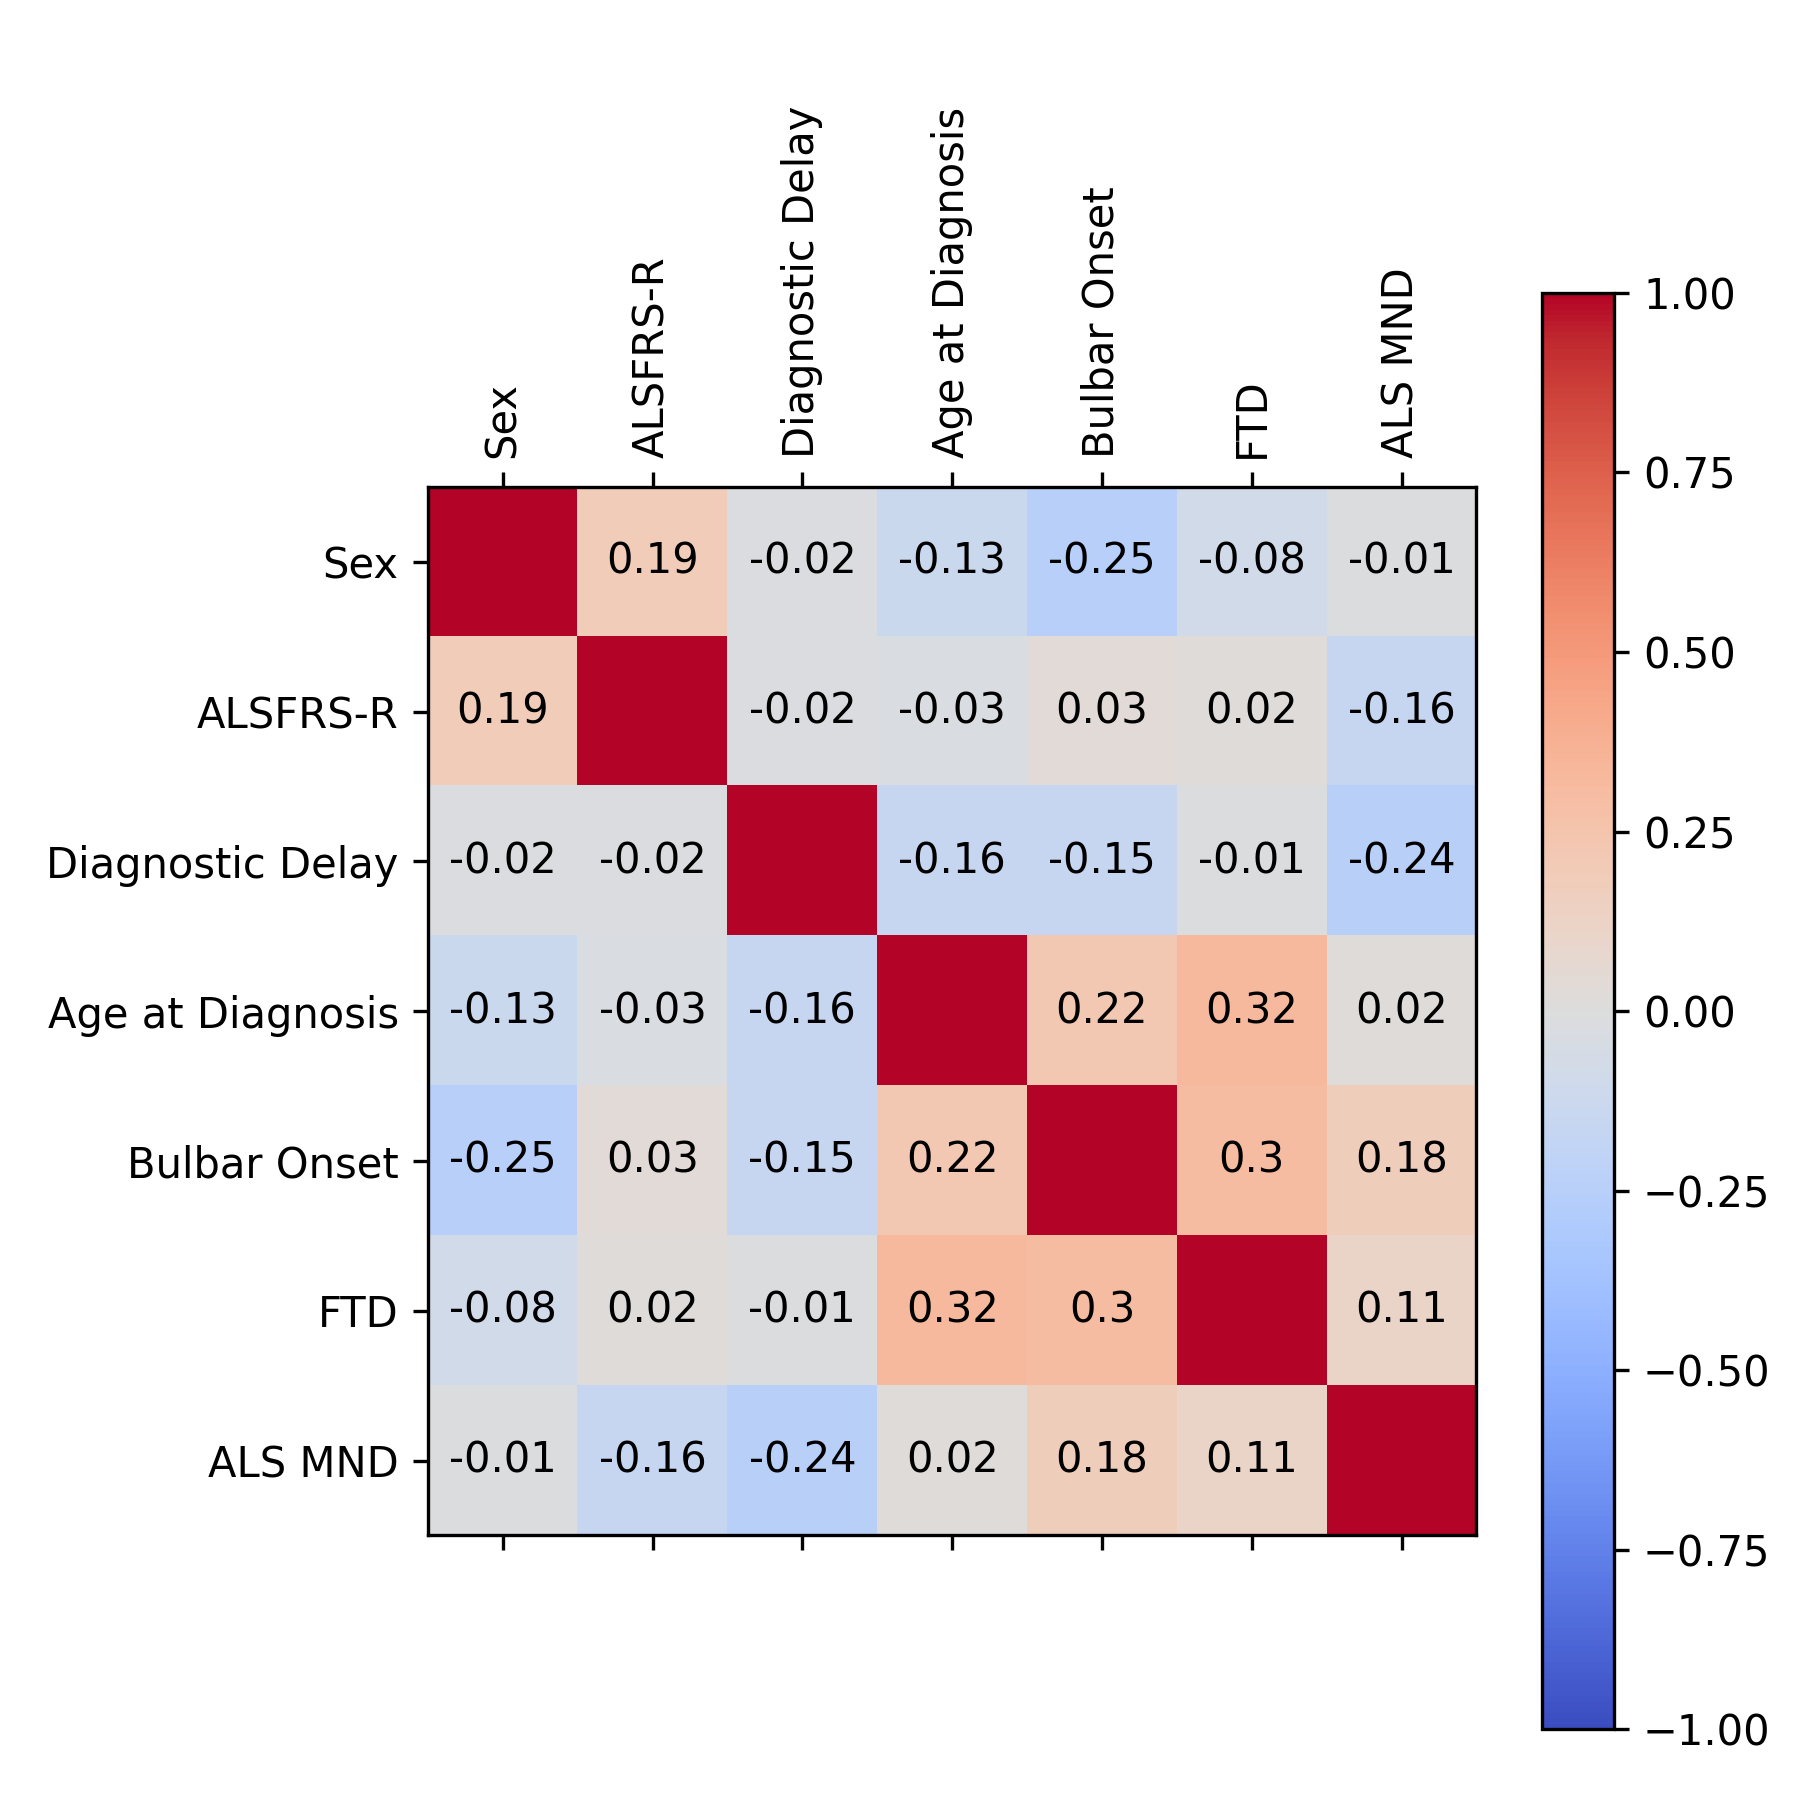
\includegraphics[width=0.75\linewidth]{figures/clinical_correlation}
    \caption{Correlation between the clinical features input into the Cox proportional hazards survival model, as calculated by Pearson's correlation coefficient.}
    \label{fig:clinicalcorrelation}
\end{figure}

The multivariable models all resulted in broken proportional hazards assumptions, which were fixed by screening the input variables by their univariable significance.
This approach is not without controversy, as it is possible that features that are not significant univariably are significant in the multivariable model.
However, we did not find this to be the case in our analysis, since the screened imaging and multimodal models resulted in more significant features than the unscreened models.

The multivariable imaging model resulted in some clinically unintuitive results, such as reported significantly harmful effects of larger cerebral white matter volume and larger volume of the thalamus.
In the univariable analysis, larger thalamus volume was significantly protective, and larger cerebral white matter volume was not significantly associated with survival.
Moreover, previous work suggests that atrophy in the thalamus suggests faster disease progression, although this is not necessarily associated with survival~\cite{sendaStructuralMRICorrelates2017,dieckmannCorticalSubcorticalGrey2022}.
By its nature, the regional brain volumes are highly correlated, which increases the risk of collinearity in the model.
Collinearity can lead to unstable estimates of the coefficients, and possibly explain a variable effect switching from harmful to protective or vice versa.

One way to mitigate the effect of collinearity in the model is to use dimensionality reduction techniques, such as principal component analysis (PCA), to reduce the number of features in the model.
Westeneng and colleagues used this technique to group the brain into larger regions based on their principal components before applying to a survival analysis model~\cite{westenengSubcorticalStructuresAmyotrophic2015}.

Diagnostic delay and FTD lost significance in the multivariable clinical model (both screened and unscreened) when age at diagnosis was included.
This lost significance could be explained by the correlations in the clinical features, shown in Figure~\ref{fig:clinicalcorrelation}.
In multivariable models, the features that are correlated with other features are less likely to be significant, because the effect of the correlated features is already accounted for by the significant features.
Figure~\ref{fig:clinicalcorrelation} shows that age at diagnosis is the most positively correlated with FTD, which could explain why FTD lost significance in the clinical model when age at diagnosis was included, and age at diagnosis remained significant.
Moreover, diagnostic delay is the most negatively correlated with ALS MND, which resulted in diagnostic delay losing significance, even though it was significant univariably.

The presence of the amygdala in the final multimodal significant features is interesting, since brain regions which are more commonly associated with MND, such as the brain stem, were not significant.
This could, again, be explained by the correlations between the features included in the model.
Figure~\ref{fig:multimodalcorrelations} in the appendices shows that the most negative correlation between FTD and a brain region is with the amygdala (
coefficient of -0.40), which could explain why FTD lost significance in the clinical model when the amygdala was included.
Moreover, the brain stem is highly correlated with the amygdala (coefficient of 0.60), which could explain why the brain stem lost significance in the multimodal model, even though it is implicated in lower motor neuron degeneration in MND .

Another example of this is that the age at diagnosis was not significant in the multimodal model, even though it was significant in the clinical model.
Inspecting the correlations between the clinical features and the brain volumes found that age at diagnosis is correlated with lateral ventricle volume (coefficient of 0.49), which could explain why age at diagnosis lost significance in the multimodal model when lateral ventricle volume was included.

The absence of these clinical variables in the imaging multivariable CPH may have led to the model picking up on brain structure not directly influencing survival, but markers of clinical features that are influencing survival.
For example, older age at diagnosis, which is associated with brain atrophy, and FTD, which is associated with limbic atrophy leading to three limbic structures being found as significant: thalamus, amygdala, and caudate.
The multimodal CPH mitigated the effect of the model picking up on brain structure not directly influencing survival, because we included the clinical features that are influencing survival into the model as well.
However, the trade-off was that the collinearity within the brain volumes but also between the brain volumes and the clinical features was high, which could mean that individual volumes are picked out as significant over clinical features and vice versa, even if both are influencing survival.

Finally the fit statistics in Table~\ref{tab:coxfitmetrics} show that the fit improved with multimodal features.
Although adding more features to a survival model is likely to increase its fit metrics, AIC also considers the number of features in the model in its calculation, so it can be concluded that the multimodal features are adding more information to the model than the clinical or imaging features alone.

%\begin{itemize}
%    \item It could also be that the model is picking up on brain structure not directly influencing survival, but markers of clinical features that are influencing survival, such as older age at diagnosis, which is associated with brain atrophy, and FTD, which is associated with limbic atrophy.
%    \item Interesting that limbic structures were being picked up as significant: thalamus, amygdala, and caudate. This could be because they are involved with cognitive and behavioural changes, which is a significant factor in MND survival, and was shown to be significant univariably with co-presence of FTD.
%\end{itemize}
%
%This correlation-driven loss of significance was also seen in the multimodal models.
%\begin{itemize}
%    \item Combining the clinical and imaging measures into one model should mitigate the effect of the model picking up on brain structure not directly influencing survival, because we will be including the clinical features that are influencing survival into the model as well
%%    \item Remaining clinical features are consistent with literature, but age at diagnosis was no longer significant.
%%    \item A marker of an aging brain is general atrophy, which can be shown by larger lateral ventricles, so it's possible that the model is picking up on the same information from the brain structure as it is from the age at diagnosis, because the lateral ventricles are significant in the multimodal model.
%%    \item Inspecting the correlations between the features found that age at diagnosis is correlated with lateral ventricle volume (coefficient of 0.49).
%%    \item Moreover, FTD has the most negative correlation with amygdala out of all the brain regions (coefficient of -0.40), which could explain why FTD lost significance in the clinical model when amygdala was included.
%%    \item Surprising that the brain stem is not significant in the multimodal model, because it is often implicated in MND survival but it has high correlation with the amygdala (0.6) so this is likely why it lost significance.
%    \item Fit statistics: fit improved with multimodal features - this could be just because we're adding more features, but it could also be because we're adding more information. AIC takes number of features into account, so it's not just that we're adding more features in the multimodal model.
%\end{itemize}
\subsection{Limitations}
The counter-intuitive results in the imaging multivariable model were likely due to limitations in this analysis.
Firstly, the sample size was relatively small ($n=125$), which could mean that the results were due to cohort-specific factors.
Moreover, the data came from two studies and multiple sites, and no harmonisation was performed to account for site-specific factors, although an argument could be made that removing site-specific factors could remove important information about the disease.
Further work could be done to investigate the effect of the sites on the results, such as by including site as a variable in the model.

Secondly, the scans were not generally taken at the same time as diagnosis, which could mean that the brain volumes are not representative of the patient's brain at the time when the clinical features were recorded.
MND is a fast-progressing disease and allowing for 12 months either side of diagnosis for including the scan is a wide window.
However, this wide window was a trade-off between sample size and data quality.
In the future, we aim to increase the sample size, which would allow us to look at scans taken closer to diagnosis to check the consistency of the results.

The collinearity of the brain volumes introduced instability into the model.
The summing of the left and right regions was done to mitigate this, but this could have also introduced information loss if the left and right regions were not equally important to survival.
Future work to mitigate this further would be to implement dimensionality reduction techniques before inputting the brain volumes into the model.

Finally, the univariable screening of the features could have introduced bias into the model, as it is possible that features that are not significant univariably are significant in the multivariable model.
Although we did not find this to be the case, there are other ways to attempt to fix the proportional hazards assumption, such as using time-dependent covariates or stratifying the model by a variable, and there are other ways to screen the features, such as using a LASSO regression to select the most important features.

%Take home message:
%\begin{itemize}
%    \item Using imaging-derived feature with clinical features increases concordance, more information into the model is better, makes the clinical measure significant as well when it wasn't before
%    \item Would this result also be sustained when using more sophisticated machine learning models? Instinct says yes because they can handle more features and more complex relationships between features - perhaps collinearity of the brain volumes would not be such an issue
%\end{itemize}

\section{Conclusion}

In this chapter, we have shown that both brain region volumes and clinical features were significantly associated with survival in MND, and that including both data modalities in a survival model increased the model's fit metrics.
The clinical features that were significantly associated with survival were consistent with the existing literature, but some of the imaging features were not, until the clinical features were included in the model.
This suggests that incorporating imaging-derived features with clinical features is a valuable approach to survival analysis in MND, and that the multimodal model is more informative than the clinical or imaging models alone.

The issues encountered during the analysis were likely due to the collinearity of the brain volumes and the correlations between the brain volumes and the clinical features.
Future work will aim to address these issues by extending this analysis to include dimensionality reduction and improved clinical characterisation of the patients, as well as increased sample size.